\chapter{League Requirements}\label{chap:league-requirements}

\section{Competition Area}

\subsection{Field Info}
\begin{itemize}
    \item Number of Fields: 2 (+1 DSPL)
    \item Space per field: \qty{90}{\meter\squared}
    \item Total gross space: \qty{180}{\meter\squared} (+\qty{90}{\meter\squared} DSPL)
\end{itemize}

\begin{figure}[H]
	\centering
	\subfloat[3D visualization]{
		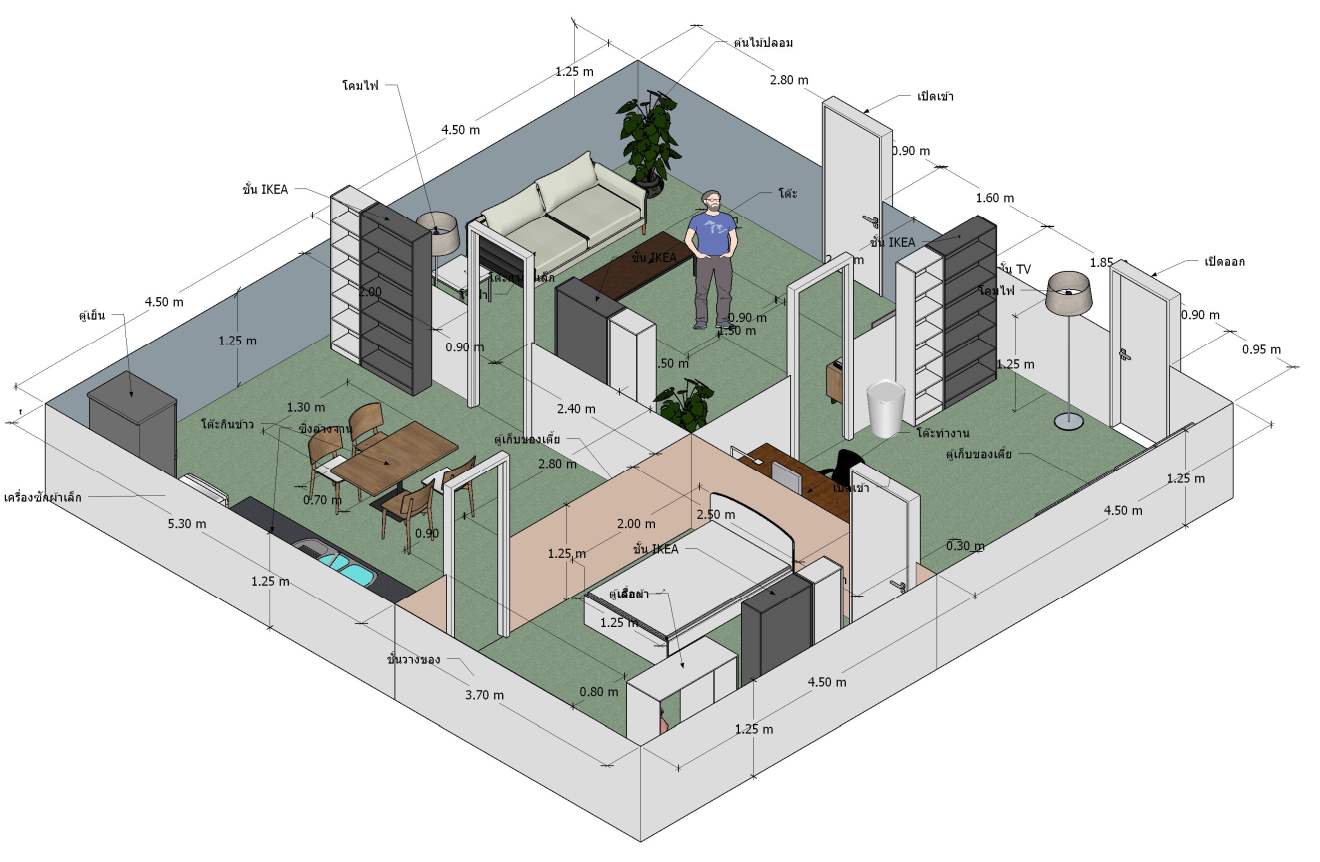
\includegraphics[width=0.48\textwidth]{images/league-arena_example3d.png}\label{fig:sample_arena_setup3d}}
	\subfloat[2D plan]{
		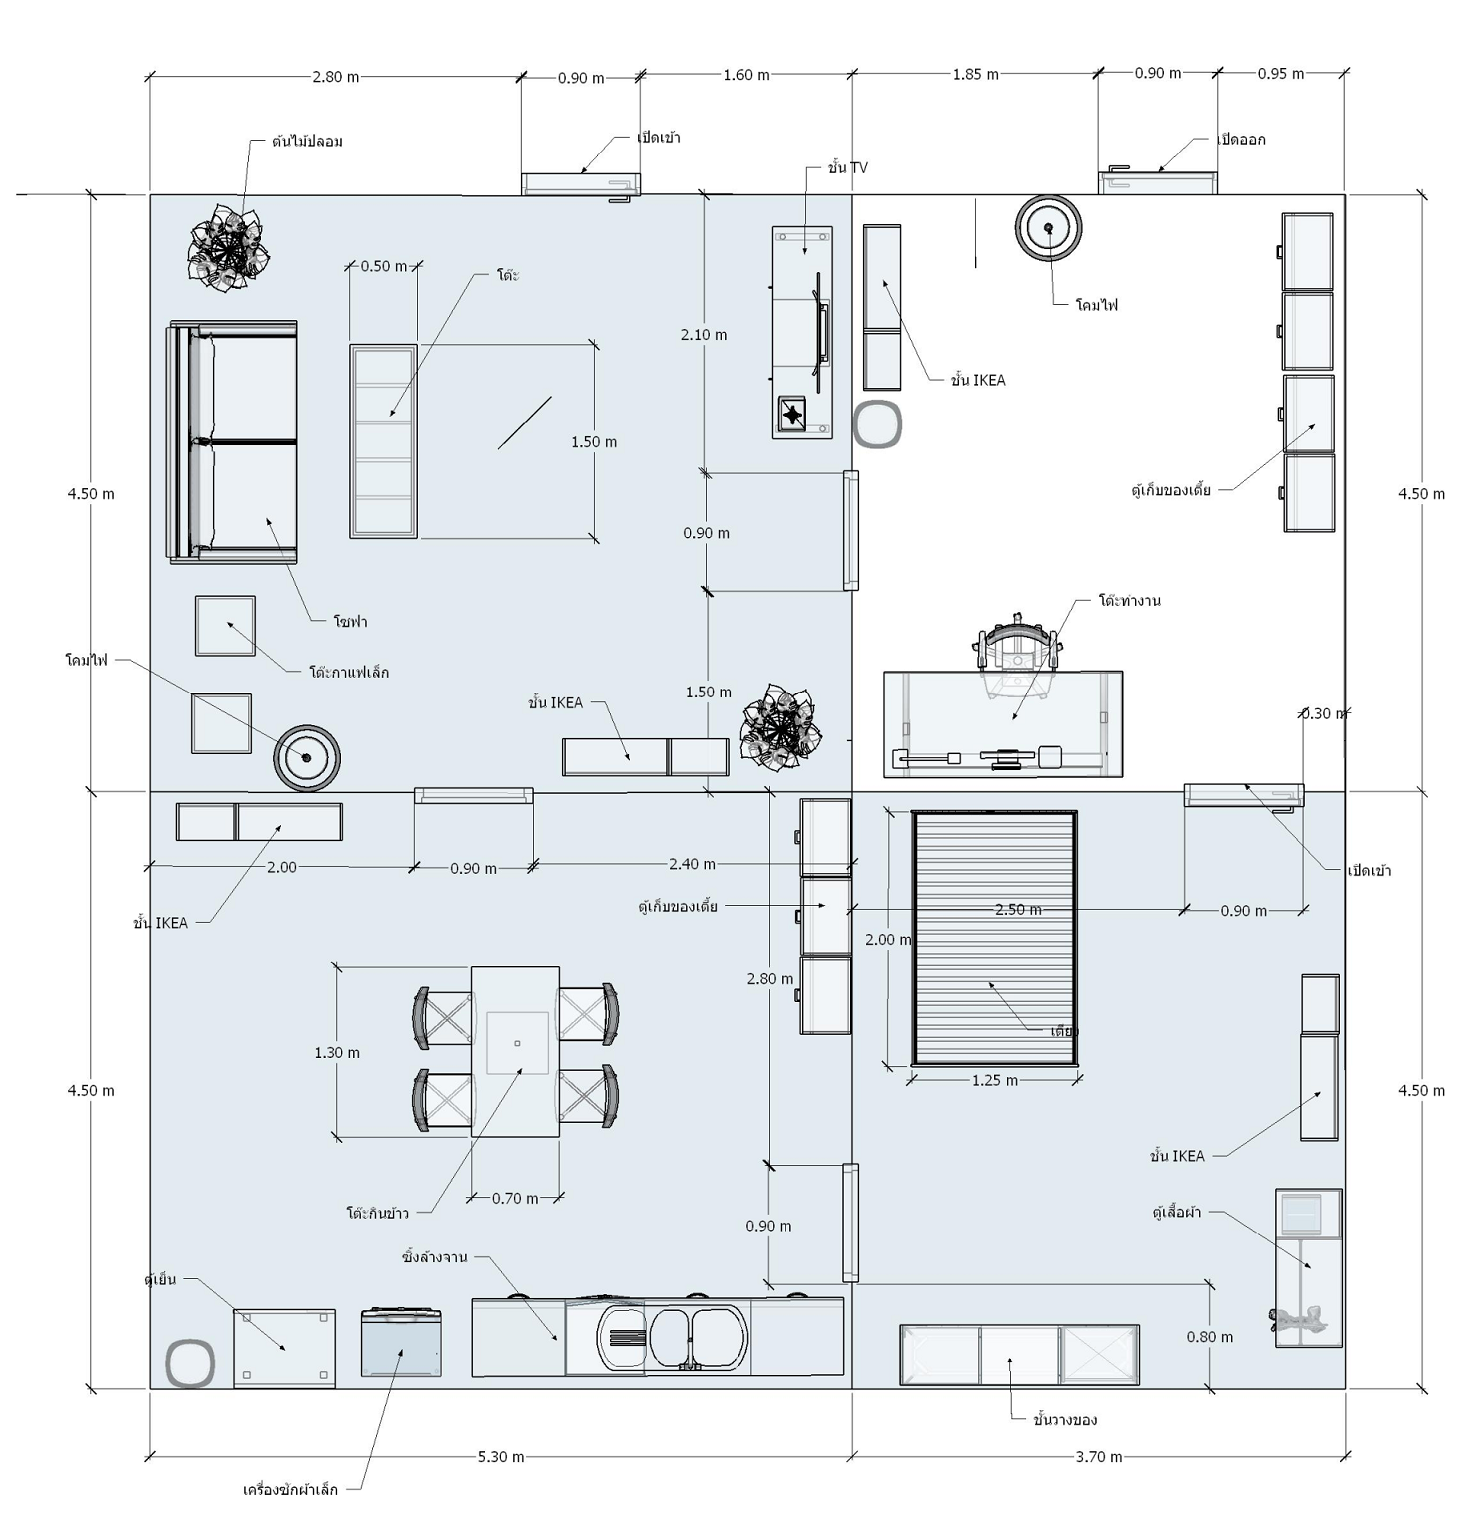
\includegraphics[width=0.48\textwidth]{images/league-arena_example.png}\label{fig:sample_arena_setup2d}}
	\caption{Sample Arena Setup}
	\label{fig:sample_arena_setup}
\end{figure}

\subsection{Detailed Setup}
The RoboCup@Home Arena is a realistic home setting (an apartment) consisting of interconnected rooms. A typical \Arena{} setup is shown in~\reffig{fig:sample_arena_setup}. The minimal configuration consists of:
\begin{itemize}
    \item a bedroom,
    \item a dining room,
    \item a living room, and
    \item a kitchen.
\end{itemize}

There are usually two OPL arenas and one DSPL arena. Sometimes, one of the OPL arenas is shared between DSPL and OPL depending on the number of participating teams in each league.

Each arena requires a dedicated WLAN access point for teams during their competition runs (more details in the next section). The indoor home setting is surrounded by high and low walls built using standard fair construction materials.

\paragraph{Dimensions} Arenas are typically around \qtyrange{90}{100}{\metre\squared}, with rooms approximately \qtyproduct{4.5 x 4.5}{\metre}. However, as little as \qty{80}{\metre\squared} is acceptable, provided there is sufficient space for robot movement. (Note: The robot base diameter is about \qty{70}{\centi\metre}, with possible extensions for arms.)

\paragraph{Walls} Walls are fixed and cannot be modified during the competition. The minimum wall height is \qty{60}{\centi\metre}; there is no maximum height, but visibility for the audience must be ensured.

\paragraph{Doors} Inside the arena, rooms are connected by door openings and/or internal doors. Each arena should have:
\begin{itemize}
    \item At least one entrance door (opening inward).
    \item At least one exit door (opening outward).
    \item All doors have handles, not knobs, and can be closed.
    \item Minimum door width: \qty{90}{\centi\metre}, height: \qty{200}{\centi\metre}.
\end{itemize}
If such doors are not feasible, alternative solutions can be discussed in advance.

\paragraph{Floor} The floor is even, with minor irregularities such as carpets or transitions between different materials. It should not be excessively slippery. There should be at least one meter of free space around the arena walls for robots to line up.

\paragraph{Appearance} The floor and walls are mostly monochromatic but may include textures such as carpets or posters.

\paragraph{Additional Setup} A table should be placed outside the arena for external computing devices for the active team.

\subsection{Sponsor Requirements}

These additional requirements are not mandated by the rules but based on request of sponsors.

\paragraph{Stairs (for humanoid robots, if applicable)} If humanoid robots participate, an external set of stairs is required. The stairs should preferably have:
\begin{itemize}
    \item 6--7 steps going up, a landing, and 6--7 steps going down.
    \item Minimum width: \qty{91}{\centi\metre}, tread depth: at least \qty{28}{\centi\metre}, riser height: \qtyrange{10}{18}{\centi\metre}(typically \qty{17.4}{\centi\metre}).
    \item Close risers for robot safety.
\end{itemize}s
Alternatively, if venue stairs meet these requirements and are near the @Home area, they may be used.

\section{Environment Requirements}
The arena is decorated to resemble a typical apartment, including:
\begin{itemize}
    \item Plants, mirrors, paintings, posters, plates, picture frames, clocks, candles with holders, and books.
\end{itemize}

\paragraph{Furnishings} The minimal setup includes:
\begin{itemize}
    \item a bed,
    \item a couch,
    \item a small table (coffee/side),
    \item a small dining table with two chairs,
    \item a trash bin,
    \item a bookcase (or other shelf-like furniture) in which objects can be placed, such that the minimum distance between shelves is \qty{30}{\centi\meter}. Two side by side doors blocking the access to at least the lower three of the shelves. The doors require U-shaped handles.
\end{itemize}

\paragraph{Kitchen} The kitchen contains:
\begin{itemize}
    \item a dishwasher,
    \item a sink,
    \item a pantry (a tall cupboard with shelves and doors with U-shaped handles).
\end{itemize}

\paragraph{Optional} Optional furnishings:
Although not strictly required, the following additional furnishings are recommended to meet expected standards and improve the overall functionality of the space:
\begin{itemize}
    \item a bigger dining table with 4 chairs instead of a small one
    \item additional (side/coffee/couch) tables,
    \item a refrigerator (with some cans and plastic bottles), and
    \item a microwave,
    \item a coat rack.
    \item a open cupboard or a small table with a television and remote control,
    \item a cupboard,
    \item a chest of drawers with at least two drawers that are between \qty{90}{\centi\meter} and \qty{120}{\centi\meter} from floor level. The drawers require U-shaped handles.
\end{itemize}

\section{Network}

\subsection{Wireless Communication}
A wireless network is provided for each arena; however, reliability is not guaranteed. The following rules apply:
\begin{itemize}
    \item Only the official arena network may be used during testing.
    \item Only the team currently active in the arena is permitted to use the network.
    \item Each team has a separate VLAN with its own SSID/password.
    \item The networks are connected to both the Internet and a wired connection available near each arena.
    \item The use of unauthorized networks (including smartphone hotspots) is strictly prohibited and may result in disqualification.
\end{itemize}

\section{Best Practices}
\begin{itemize}
    \item One entry door should open inward; one exit door should open outward.
    \item Avoid loose cables and large uneven surfaces.
    \item Arrange DSPL and OPL team tables near their respective arenas.
\end{itemize}

\section{Additional Equipment}
The minimum object set required includes:
\begin{itemize}
    \item Local light (\qty{0.5}{\kilogram}) household objects of different categories such as, but not limited to: Drinks, Snacks, Food, Fruits, Toys, Cleaning Supplies
    \item Tableware: dish, bowl, cup/mug, napkin.
    \item Cutlery: fork, knife, spoon.
    \item Trash bags: large plastic bags with handles.
    \item Bags: lightweight with vertical handles.
    \item Trays: for bi-manual manipulation.
    \item Pourable objects: e.g., a cereal box.
    \item Heavy objects: \qtyrange{1}{1.5}{\kilogram}.
    \item Tiny objects: \qty{5}{\centi\meter} (e.g., paper, teabag, pen).
    \item Fragile objects: easily breakable (e.g., a chocolate egg).
    \item Deformable objects: flexible (e.g., cloth).
    \item Garbage bag: a tieable garbage bag.
\end{itemize}

\section{League Organization Area}
\paragraph{OC Requirements} The \OC{} area must include the following::
\begin{itemize}
    \item \numrange{2}{3} tables, each accompanied by two chairs
    \item Access to power outlets and a LAN connection
    \item Access to a printer (unless paperless setup is in place).
    \item A mobile display connected to the table; if unavailable, a poster stand or announcement board may be used as an alternative
\end{itemize}

\section{Teams Area}
\paragraph{Participation Area} Each team should have:
\begin{itemize}
    \item One table per four members, with chairs.
    \item At least one power outlet and one Ethernet connection.
    \item \qty{2}{\metre\squared} for robot storage, \qtyrange{1}{2}{\metre\squared} for robot handling.
    \item \qtyrange{4}{5}{\metre\squared}  near the team area for handling the robot.
    \item Adequate space between table rows for robot transport.
\end{itemize}

\section{Others}
\begin{itemize}
    \item New Changes: SSPL has been dissolved.
    \item Additional information: TBD.
\end{itemize}

